\documentclass[a4paper, 11pt]{article}

%%% Zeichenkodierung, Rechtschreibung und Umlaute
\usepackage[utf8]{inputenc}
\usepackage[ngerman]{babel}
\usepackage[T1]{fontenc}

%%% Mathematische Symbole, Gleichungen
\usepackage[fleqn]{amsmath}
\usepackage{amsfonts}
\usepackage{amssymb}
\usepackage{amsthm}
\usepackage{mathtools}
\usepackage{bm}
%\usepackage{colonequals} % Zusätzliche Relationssymbole

%%% Tabellen
\usepackage{tabularx}
\usepackage{array}
\usepackage{multicol}
\usepackage{float}

%%% Seitenformat und -ränder
%%% -Alternative 1-
\usepackage{geometry}
\geometry{a4paper, top=25mm, bottom=20mm, left=20mm, right=20mm}
%%% -Alternative 2-
%\usepackage[headheight=110pt]{geometry}
%\geometry{a4paper,left=30mm,right=30mm, top=35mm, bottom=30mm}

%%% Seitenstile (Kopf- und Fußzeile)
\usepackage{fancyhdr}
\pagestyle{fancy}

%%% Sonstiges
\usepackage{caption} % Untertitel von Grafiken/Tabellen manipulieren
\usepackage{enumerate} % Aufzählungszeichen ändern
\usepackage{graphicx} % Standarderweiterung für Bilddateien
\usepackage{hyperref} % Hyperlinks
\usepackage{lastpage} % Berechnung der Seitenzahl
\usepackage{polynom} % Polynomdivision
\usepackage{setspace} % Zeilenabstand
%\usepackage{textgreek} % griechische Symbole
\usepackage{tikz} % Umfassendes Tool, um Grafiken zu erstellen
\usepackage{verbatim} % Schreibmaschinen-Stil (für Code-Ausschnitte)
\usepackage{float}

%%% Eingaben (z.B. für das Deckblatt)
\newcommand{\moduleabrv}{EDS Gruppe 15}
\newcommand{\module}{Konfigurierbare eingebettete Systeme}
\newcommand{\semester}{Beuth Hochschule - Wintersemester 2018/19}
\newcommand{\finishingdate}{12.11.2018}
\newcommand{\titletextabrv}{       KES}
\newcommand{\titletext}{Laborübung 1}

%%%-- Für das Deckblatt --
\title{
	~\\[4cm]
	\textbf{
		\module\\[0.25cm]
		\normalsize \semester \\[1.5cm]
		\Huge\titletext\\
	}
}

\author{
  \vspace{3.5cm}\\
  \begin{tabular}{l}
    \textbf{Gruppe 15:}\\\hline
    Omid Rahimian Mashhadi Mat.Nr.: 872958\\
    Torsten Michael Schenk Mat.Nr.: 838995\\
  \end{tabular}
}

\date{
	\vfill
	Abgabedatum: \finishingdate\\
	\vspace{5mm}
	Seitenanzahl: \pageref{LastPage}
}

%%% -- Kopf- und Fußzeile --
%%% Kopfzeile linker Bereich
\lhead[\leftmark]{\textbf{\moduleabrv}}
%%% Kopfzeile mittlerer Bereich
\rhead[\rightmark]{\rightmark{\titletextabrv}}
%%% Kopfzeile linker Bereich
%%\rhead{\textbf{zum \finishingdate}}
%%% Fußzeile
\cfoot{\thepage  \ / \pageref{LastPage}}

%%% Serifenfreie Fonts benutzen
%\renewcommand{\familydefault}{\sfdefault}

%%% Font
\usepackage{charter}

%%% Tiefe der Einrückung nach Absätzen
\setlength{\parindent}{0pt}

%%% Evtl. Änderungen des Typs einer Aufzählungsebene (z.B. zur Anpassung an das Aufgabenblatt)
%\renewcommand{\labelenumi}{\alph{enumi})}
%\renewcommand{\labelenumii}{(\roman{enumii})}
%\renewcommand{\labelenumiii}{\arabic{enumiii}.}
%\renewcommand{\labelenumii}{\textbf{-}}

\begin{document}

%%% Deckblatt
\maketitle
\thispagestyle{empty} % Keine Seitenzahl hier

\newpage
%\renewcommand\contentsname{Inhalt}
%\tableofcontents
    {\pagestyle{plain}
    \tableofcontents
    \cleardoublepage
    }

%\newpage
%%% Seitenzahl zurücksetzen
%\clearpage
%\setcounter{page}{1}

%%% Zeilenabstand
%\singlespacing
\onehalfspacing
%\doublespacing

%%%-- Eigentlicher Inhalt --
\section{Vorwort}
Bei der Recherche zur Bearbeitung der Übungen wurden viele englischsprachige Webseiten zu rate gezogen. Generell kann man sagen, dass englische Fachbegriffe sich im Bereich FPGA und embedded Design etabliert haben, so dass eine Übersetzung eher verwirren als helfen würde. Daher haben wir uns entschieden, die \textbf{englischen} Bezeichner und Beschreibungen beizubehalten.\\
Um Codeabschnitte besser von Beschreibungen besser unterscheiden zu können, wurde eine eigene Schriftart verwendet:
\begin{verbatim}
  Kommandozeilen Eingaben und Codesnippets werden wie HIER dargestellt.
\end{verbatim}

\section{Aufgabe 1} \label{ex1}
In der Laborübung wurde das ZedBoard Zynq-7000 eingesetzt. Es umfasst als \textbf{PL} den Artix-7 FPGA mit 85K Logic Cells (Device Z-7020, Part: XC7Z020) und als \textbf{PS} den Dual-core ARM Cortex-A9 MPCore™ mit 866 MHz.

\begin{minipage}{\textwidth}
    \begin{center}        
        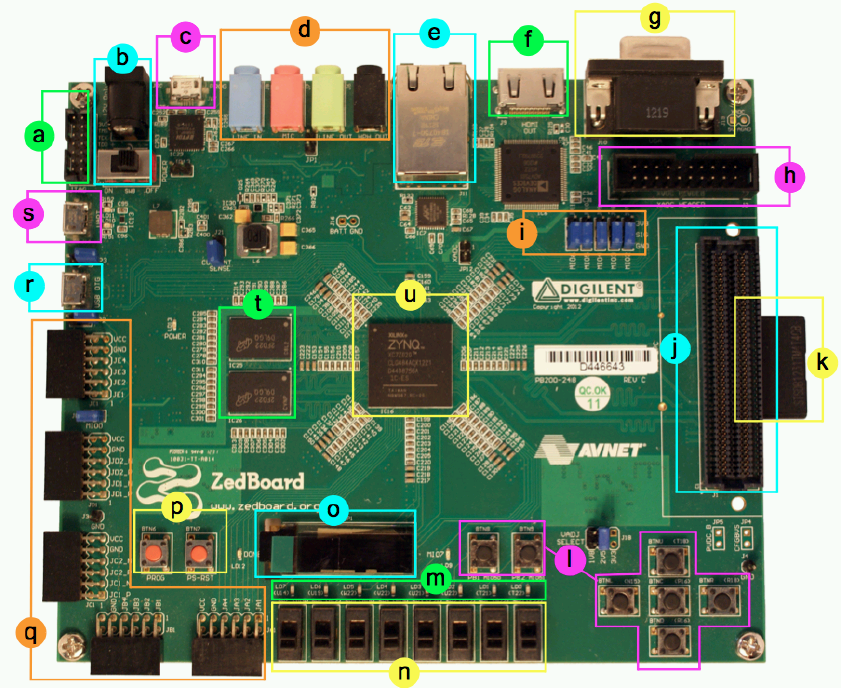
\includegraphics[scale=0.5]{img/a1.png} 
    \end{center}
\end{minipage}
\begin{center}
ZedBoard mit Xilinx Zynq-7000 SoC
\end{center}

Wichtigste Anschlüsse für Laborübung 1
\begin{itemize}
\item b) Netzanschluss
\item c) USB-JTAG (Programmierung)
\item s) USB-UART (serielle Schnittstelle)
\item g) \textbf{VGA-Port} (Display)
\item i) Jumper (Konfiguration eines Programmierungsanschlusses )
\end{itemize}

\subsection {VGA-Controller Theorie}
Die Aufgabe bestand darin einen VGA-Controller in VHDL Entities zu entwickeln. Das Schaubild zeigt die Strukturierung 
des Blockdesigns. Der rot umrandete Block war eigenständig zu entwerfen und zu implementieren. \\
\begin{minipage}{\textwidth}
    \begin{center}        
        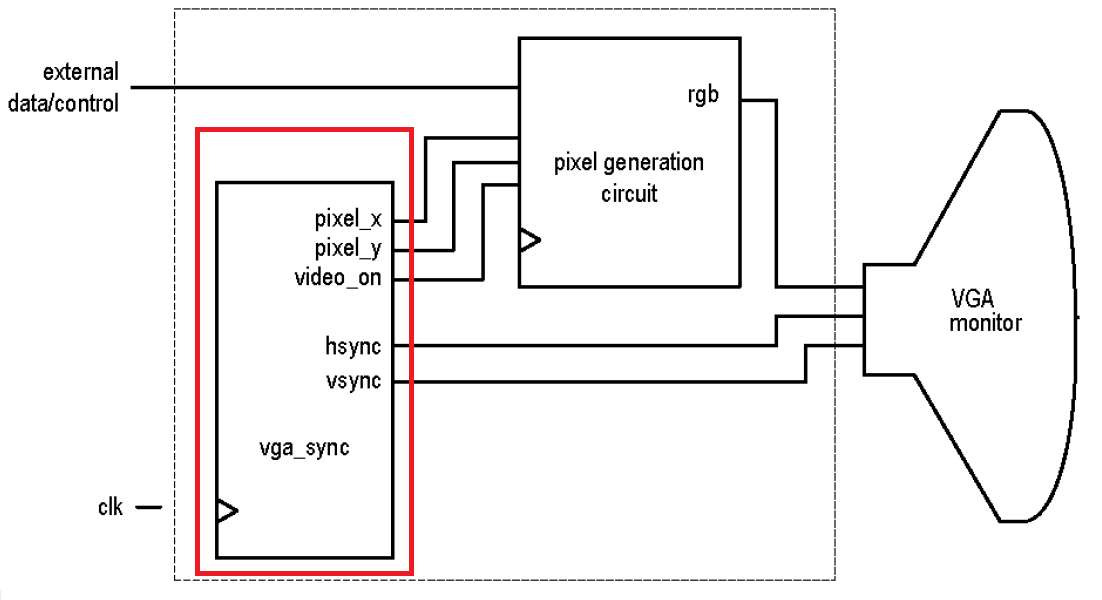
\includegraphics[scale=0.5]{img/vga_contr.png} 
    \end{center}
\end{minipage}
\begin{center}
VGA Controller Schema
\end{center}

\begin{minipage}{\textwidth}
    \begin{center}        
        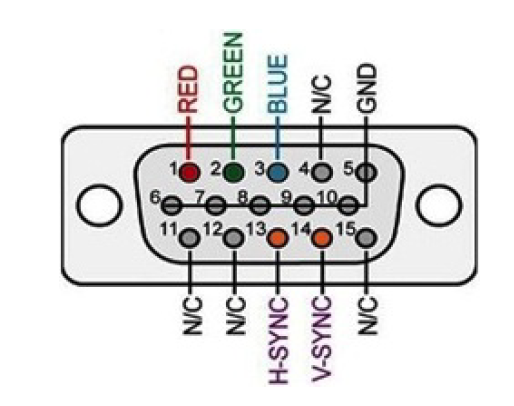
\includegraphics[scale=0.5]{img/vgaport.png} 
    \end{center}
\end{minipage}
\begin{center}
VGA Portbelegung
\end{center}

Das VGA-Signal besteht aus dem sichtbaren Bildbereich. Hier 640*480px und dem Front- und Backporch Bereich, der in vergangener 
Zeit dazu diente den Elektronenstrahl zu lenken. Insgesamt sind inklusive aller Bereiche 800*525 mit dem VGA-Signal zu takten.\\
Um die Clock-Geschwindigkeit zu berechnen wird eine Bildaufbaufrequnz von 60Hz angestrebt. \\
800*525*60 = 25,2 M Pixel/s.\\

\begin{minipage}{\textwidth}
    \begin{center}        
        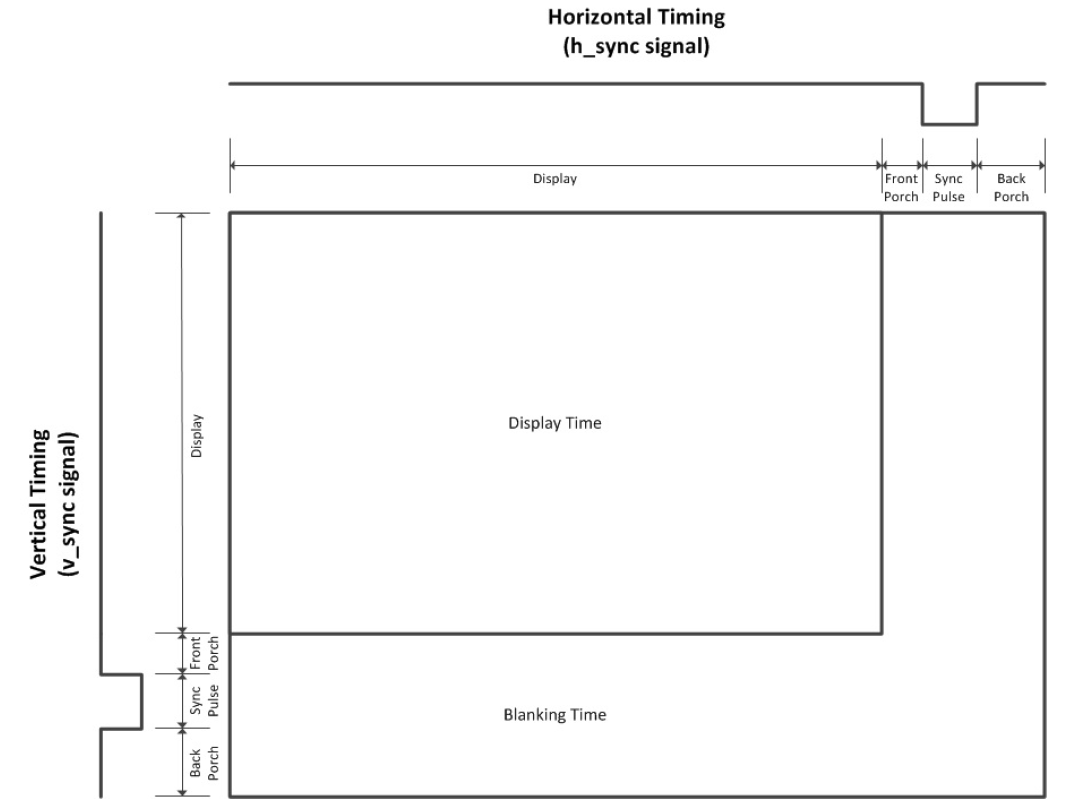
\includegraphics[scale=0.5]{img/porch.png} 
    \end{center}
\end{minipage}
\begin{center}
VGA Bildbereich und Porches
\end{center}

\subsection{VGA-Controller Implementation}
Hier wird das Vivado Block Diagramm dargestellt, mit sys\_clock im unteren rechten Bereich (100MHz) so wie dem clk\_wtz\_0 um 
die Clock auf 25.172 MHz zu reduzieren. Der util\_vector\_logic\_0 negiert das locked Signal und kann so als Reset Signal für die VGA\_Controller verwendet werden.\\

\begin{minipage}{\textwidth}
    \begin{center}        
        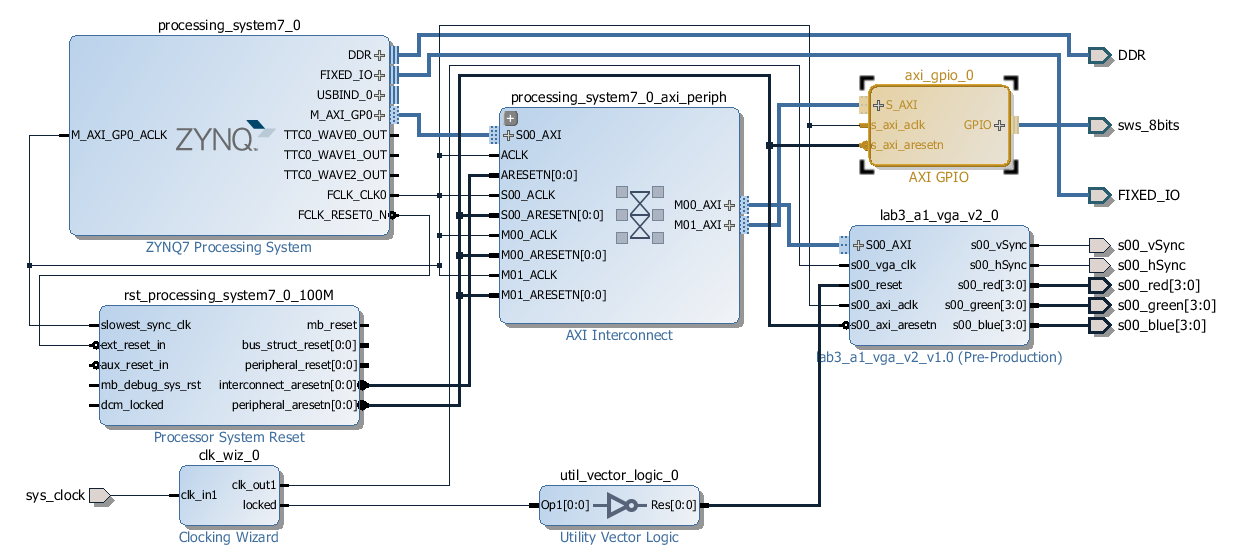
\includegraphics[scale=0.5]{img/block_a2-switches.png} 
    \end{center}
\end{minipage}
\begin{center}
Vivado Blockdiagramm
\end{center}

Als Beispielanzeige der Simulation mit den Testdaten (reduzierte Bildgröße) wurde ein  Bereich imunteren Porch-Bereich ausgewählt. Sobald vsync `0' ist werden die Pixelzähler wieder auf (0,0) für den nächsten Frame zurückgesetzt. Die zwei rund markierten Signalbereiche stellen die hsync Signale dar, die auch gesetzt werden, wenn das vsync Signal `0' ist. \\

\begin{minipage}{\textwidth}
    \begin{center}        
        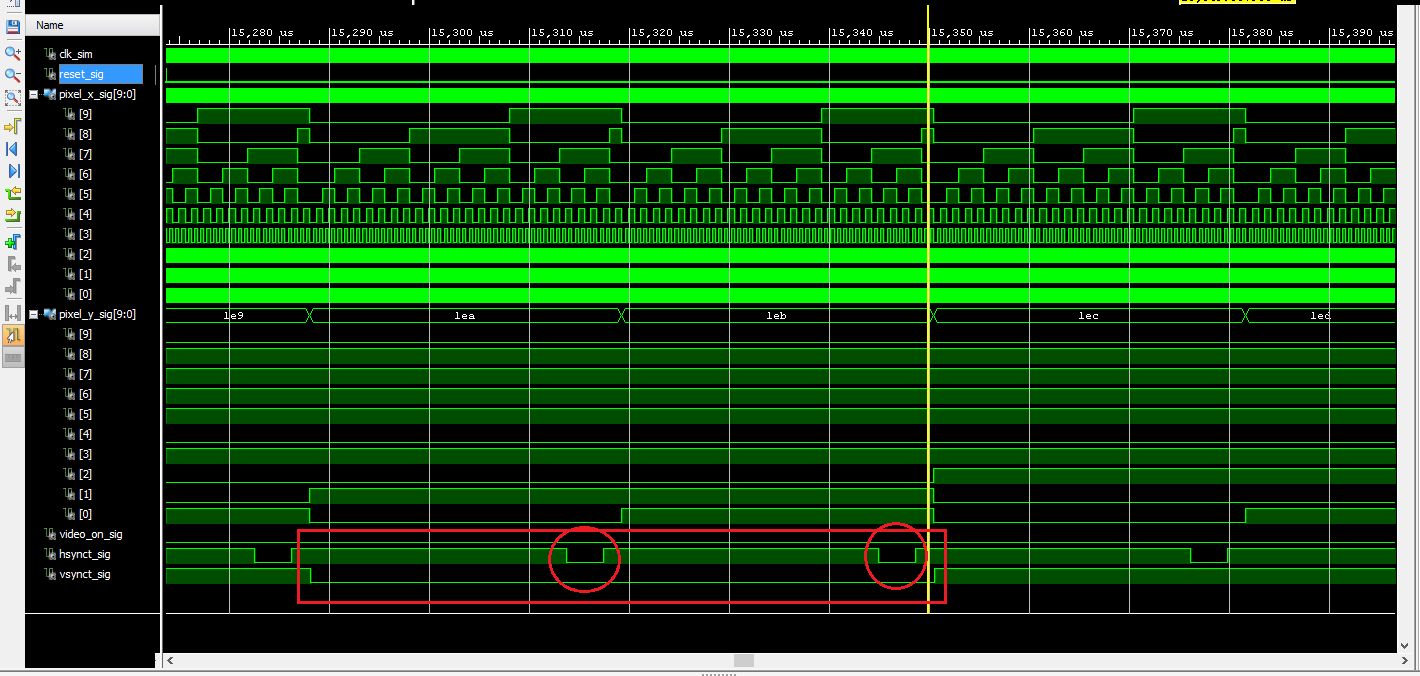
\includegraphics[scale=0.4]{img/hvsync.png} 
    \end{center}
\end{minipage}
\begin{center}
Vivado Simulation
\end{center}

Vivado Ports für die Bank 33 (3.3V), je 4 Signale gehen an die Farbkanäle und nur zwei hsync und vsync kontrollieren 
die Zeilen und Spalten.\\

\begin{minipage}{\textwidth}
    \begin{center}
        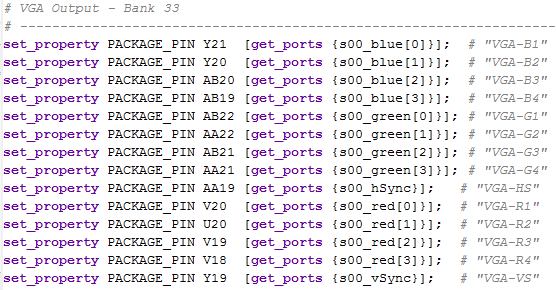
\includegraphics[scale=0.6]{img/ports_a1.png} 
    \end{center}
\end{minipage}
\begin{center}
VGA Port Belegung Vivado
\end{center}


vga\_sync Entity:
\begin{verbatim}
 ----------------------------------------------------------------------------------
-- Create Date: 09.12.2018 12:48:58
-- Module Name: vga_sync - impl
----------------------------------------------------------------------------------
library ieee;
use ieee.std_logic_1164.all;
use ieee.numeric_std.all;

-- Uncomment the following library declaration if using
-- arithmetic functions with Signed or Unsigned values
--use IEEE.NUMERIC_STD.ALL;

-- Uncomment the following library declaration if instantiating
-- any Xilinx leaf cells in this code.
--library UNISIM;
--use UNISIM.VComponents.all;

entity vga_sync is
    Port ( vga_clk   : in  std_logic;
           reset     : in  std_logic;
           pixel_x   : out std_logic_vector (9 downto 0);
           pixel_y   : out std_logic_vector (9 downto 0);
           video_on  : out std_logic;
           hSync     : out std_logic;
           vSync     : out std_logic);
end vga_sync;

architecture impl of vga_sync is
   -- REAL VGA MONITOR DATA 
    CONSTANT h_active_sig : integer := 799; -- full horizontal
    CONSTANT h_active_video  : integer := 639; -- horizontal active video
    -- CONSTANT h_front_porch : integer := 16; -- horizontal front porch
    -- CONSTANT h_retrace     : integer := 96; --horizontal retrace/sync pulse length
    -- CONSTANT h_back_porch : integer := 48; -- horizontal back porch
    CONSTANT h_retrace  : integer := 655; --h_active_video 639 + 16
    CONSTANT h_back_porch :integer := 752; --h_active_video 639+16+96 (+1 for<check)
    
    CONSTANT v_active_sig : integer := 524; -- full vertical
    CONSTANT v_active_video  : integer := 479; -- vertical active video
    -- CONSTANT v_front_porch : integer := 10; -- vertical front porch
    -- CONSTANT v_retrace  : integer := 2; -- vertical retrace / sync pulse length
    -- CONSTANT v_back_porch : integer := 33; --vertical back porch
    CONSTANT v_retrace  : integer:= 489; -- v_active_video 479 + 10
    CONSTANT v_back_porch :integer:= 492; --v_active_video 479+10+2 (+1 for<check)
   
   -- TEST SIGNALS for SIMULATION -- 
    -- CONSTANT h_active_sig    : integer := 29; -- full horizontal
    -- CONSTANT h_active_video  : integer := 19; -- horizontal active video
    -- -- CONSTANT h_front_porch  : integer := 16; -- horizontal front porch
    -- -- CONSTANT h_retrace :integer := 96; --horizontal retrace/sync pulse length
    -- -- CONSTANT h_back_porch  : integer := 48; -- horizontal back porch
    -- CONSTANT h_retrace : integer := 24; -- h_active_video 639 + 16
    -- CONSTANT h_back_porch :integer := 27; --h_active_video 639+16+96 (+1 for<check)
    -- 
    -- CONSTANT v_active_sig    : integer := 19; -- full vertical
    -- CONSTANT v_active_video  : integer := 9; -- vertical active video
    -- -- CONSTANT v_front_porch   : integer := 10; -- vertical front porch
    -- -- CONSTANT v_retrace : integer := 2; -- vertical retrace/sync pulse length
    -- -- CONSTANT v_back_porch    : integer := 33; -- vertical back porch
    -- CONSTANT v_retrace       : integer := 13; -- v_active_video 479 + 10
    -- CONSTANT v_back_porch : integer := 16; --v_active_video 479+10+2 (+1 for<check)

   signal px_reg   : unsigned(9 downto 0) := (others => '0'); -- x full 0 to 799
   signal px_next  : unsigned(9 downto 0);
   signal py_reg   : unsigned(9 downto 0) := (others => '0'); -- y full 0 to 524
   signal py_next  : unsigned(9 downto 0);
   
   signal hsync_reg  : std_logic := '0';
   signal hsync_next : std_logic;
   
   signal vsync_reg  : std_logic := '0';
   signal vsync_next : std_logic;
   
   signal video_on_reg  : std_logic := '0';
   signal video_on_next : std_logic;
   
begin
   -- IMPLEMENTATION WITH REGISTERS
    vga_count : process (vga_clk)
    begin
        if (rising_edge(vga_clk)) then
            if (reset = '1') then
                px_reg    <= (others => '0');
                py_reg    <= (others => '0');
               
                hsync_reg <= '1';
                vsync_reg <= '1';
            else
            
                -- full size counter including porches
                px_reg  <= px_next;
                py_reg  <= py_next;
                
                -- sync signalss
                hsync_reg <= hsync_next;
                vsync_reg <= vsync_next;
                
                -- video active - inactive
                video_on_reg <= video_on_next;
      
            end if;
        end if;
    end process vga_count;
    
    -- CHECK all REQUIREMENTS for sync and video_on.
    -- modulo 799
    px_next <= (others => '0') when (px_reg = h_active_sig) else px_reg + 1; 
    
    -- reset on h=799 and v=524 (max rows)
    py_next<=(others=>'0') when ((px_reg=h_active_sig) and (py_reg=v_active_sig)) else 
           py_reg + 1  when (px_reg=h_active_sig) else py_reg; -- add 1 if row finished 
    
    -- modulo 639 in col, 479 in row
    video_on_next<='0' when((px_reg>h_active_video) or (py_reg>v_active_video)) else '1'; 
    
     -- '0' from 656 to 751 (96 px)
    hsync_next <= '0' when ((px_reg > h_retrace) and (px_reg < h_back_porch)) else '1';
    -- '0' from 490 to 491 (2 px)
    vsync_next <= '0' when ((py_reg > v_retrace) and (py_reg < v_back_porch)) else '1';  
    
    -- set output from registers
    pixel_x <= std_logic_vector(px_reg);
    pixel_y <= std_logic_vector(py_reg);
    video_on <= video_on_reg;
    hSync    <= hsync_reg;
    vSync    <= vsync_reg;

end impl;
 \end{verbatim}
\section{Aufgabe 2} \label{ex2}
In der Aufgabe 2 wurde eine Fibonacci-Algorithm in c mitgebracht. Der Code wurde mit HLS synthetisiert und sowohl den Ressourcenverbrauch als auch das Timing unseres Codes analysiert.

\subsection{C-Code}
C-Code zur Berechnung des n-ten Wertes F(n) der  Fibonacci-Folge aus den Startwerten F0 = 0 und F1 = 1\\

Fibonacci für Hardware Implementation
\begin{verbatim}
#include "fir.h"

void fir (
  data_t result[20],
  data_t n
  ) {

  int i;
  *result = 0;
  *(result+1) = 1;
  Shift_Accum_Loop: for (i=2;i<20;i++) {
	  *(result+i) =  *(result+i-1) +  *(result+i-2);
  }
}
\end{verbatim}

Testbench
\begin{verbatim}
#include <stdio.h>
#include <math.h>
#include "fir.h"

int main () {
   FILE         *fp;

  data_t signal, output[N];
  //coef_t taps[N] = {2,100,9};

  int i;
  
  fp=fopen("out.dat","w");
  fir(output,N);

  for (i=0;i<N;i++) {
	// Execute the function with latest input
	// Save the results.
    fprintf(fp," the %d-Fibonatchi is =  %d\n",i+1,output[i]);
  }
  fclose(fp);

  printf ("Comparing against output data \n");
  if (system("diff -w out.dat out.gold.dat")) {

	fprintf(stdout, "*******************************************\n");
	fprintf(stdout, "FAIL: The result is not correct\n");
	fprintf(stdout, "*******************************************\n");
     return 1;
  } else {
	fprintf(stdout, "*******************************************\n");
	fprintf(stdout, "PASS: The result is correct!\n");
	fprintf(stdout, "*******************************************\n");
     return 0;
  }
}
\end{verbatim}

\subsection{C-Code Analyse}
Das Bild zeigt den Ressourcenverbrauch und das Timing\\

\begin{minipage}{\textwidth}
    \begin{center}        
        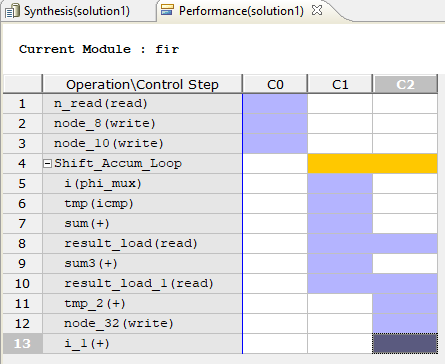
\includegraphics[scale=0.75]{img/Fibo.png} 
    \end{center}
\end{minipage}
\begin{center}
Perfomance in Zyklen
\end{center}

\begin{minipage}{\textwidth}
    \begin{center}        
        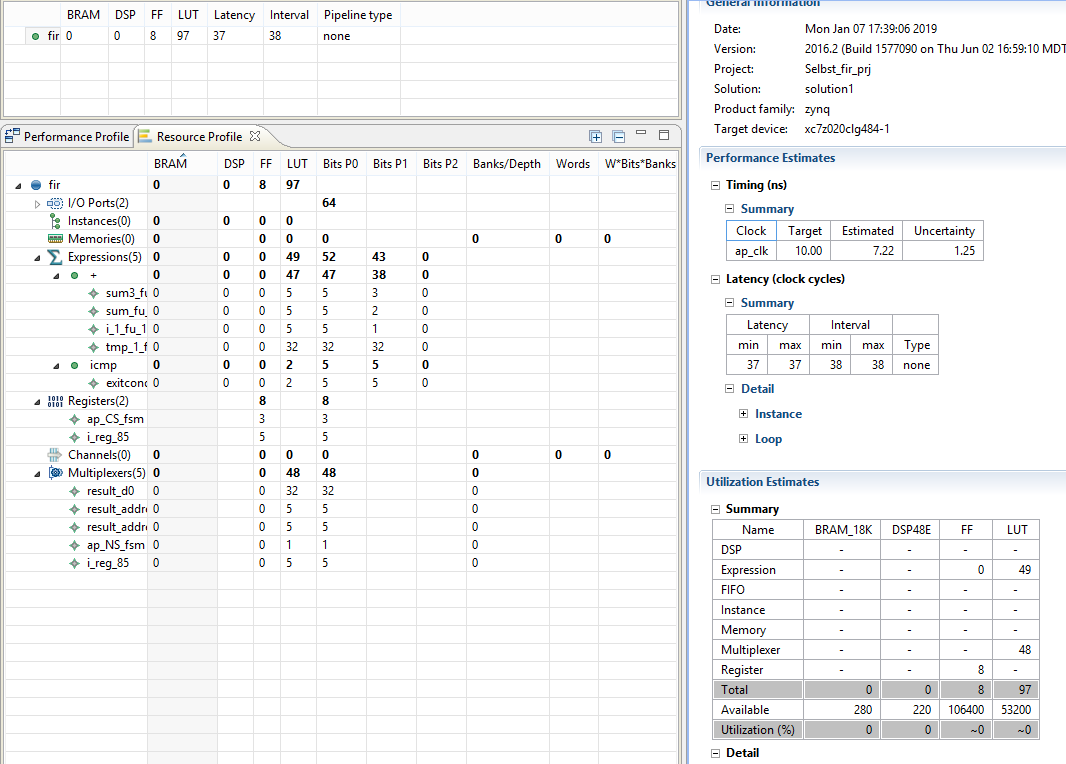
\includegraphics[scale=0.6]{img/fibo1.png} 
    \end{center}
\end{minipage}
\begin{center}
Ressourcenverbrauch 1
\end{center}

\begin{minipage}{\textwidth}
    \begin{center}        
        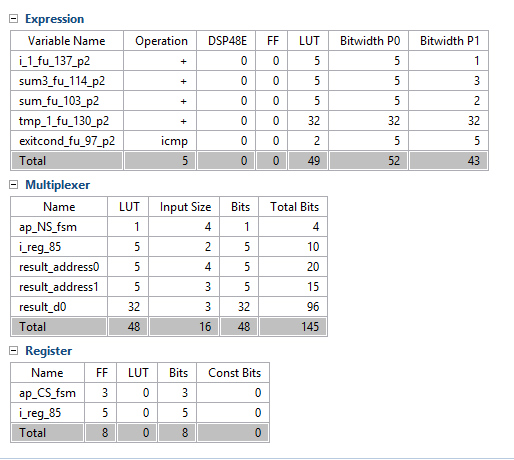
\includegraphics[scale=1.0]{img/fibo2.png} 
    \end{center}
\end{minipage}
\begin{center}
Ressourcenverbrauch 2
\end{center}




\section{Aufgabe 3} \label{ex3}

Es wurde ein Projekt mit AXI Timer und aktiviertem Interrupt als IP Core ausgewählt. Jeder Ablauf des Timers wird 
registriert und sobald dies 3 mal eintritt, die LED Anzeige als Binärzähler um 1 inkrementiert. 
Das bedeutet, die LEDs werden in Echtzeit weitergeschaltet, da der Timer in Hardware implementiert ist und nicht abhängig 
von der CPU load oder dem Thread handling ist. Auch entfällt das polling.\\

Frei nach: https://www.youtube.com/watch?v=gaZ1kRJzCok

\begin{verbatim}
  // timer presetting & reset value
  #define TMR_LOAD  0xF8000000 // 32 bit
\end{verbatim}

Blockschaltbild in Vivado\\
\begin{minipage}{\textwidth}
    \begin{center}        
        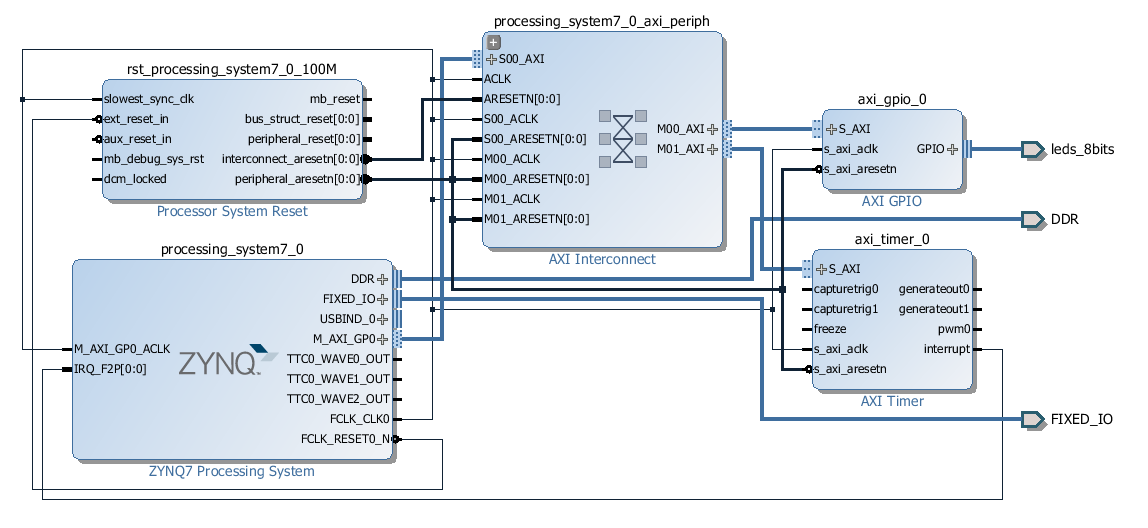
\includegraphics[scale=0.57]{img/timer3block.png} 
    \end{center}
\end{minipage}
\begin{center}
AXI Timer mit Interrupt \& AXI GPio
\end{center}


\begin{verbatim}
/*   ps7_uart    115200 (configured by bootrom/bsp) */
#include <stdio.h>
#include "platform.h"

#include "xparameters.h"
#include "xgpio.h"
#include "xtmrctr.h"
#include "xscugic.h"
#include "xil_exception.h"
#include "xil_printf.h"

// parameter definitions
#define INTC_DEVICE_ID              XPAR_PS7_SCUGIC_0_DEVICE_ID
#define TMR_DEVICE_ID               XPAR_TMRCTR_0_DEVICE_ID
#define LEDS_DEVICE_ID              XPAR_AXI_GPIO_0_DEVICE_ID
#define INTC_TMR_INTERRUPT_ID       XPAR_FABRIC_AXI_TIMER_0_INTERRUPT_INTR

#define TMR_LOAD  0xF8000000
XGpio   LEDInst;
XScuGic INTCInst;
XTmrCtr TMRInst;

// only visible to module
static int led_data;
static int tmr_count;

// Prototype functions
static void TMR_Intr_Handler(void *baseeaddr_p);
static int  IntcInitFunction(u16 DeviceID, XTmrCtr *TmrInstancePtr);

void TMR_Intr_Handler(void *baseeaddr_p) {
  if (XTmrCtr_IsExpired(&TMRInst,0)) {
    // Once it has expired 3 times, stop, increment counter
    // reset timer and start running again
    if (tmr_count == 3) {
      XTmrCtr_Stop(&TMRInst,0);
      tmr_count = 0;
      led_data++;
      XGpio_DiscreteWrite(&LEDInst, 1, led_data);
      XTmrCtr_Reset(&TMRInst, 0);
      XTmrCtr_Start(&TMRInst, 0);
    } else
       tmr_count++;
  }
}

// Initial setup functions
int InterruptSystemSetup(XScuGic *XScuGicInstancePtr) {
  // Enable interrupt
  Xil_ExceptionRegisterHandler(XIL_EXCEPTION_ID_INT,
      (Xil_ExceptionHandler) XScuGic_InterruptHandler,
      XScuGicInstancePtr);
  Xil_ExceptionEnable();

  return XST_SUCCESS;
}

int  IntcInitFunction(u16 DeviceID, XTmrCtr *TmrInstancePtr) {
  XScuGic_Config *IntcConfig;
  int status;

  // Interrupt controller initialization
  IntcConfig = XScuGic_LookupConfig(DeviceID);
  status = XScuGic_CfgInitialize(&INTCInst, IntcConfig,
  IntcConfig->CpuBaseAddress);
  if (status != XST_SUCCESS)
    return XST_FAILURE;

  // Call to interrupt setup
  status = InterruptSystemSetup(&INTCInst);
  if (status != XST_SUCCESS)
    return XST_FAILURE;

  // Connect timer interrupt to handler
  status = XScuGic_Connect(&INTCInst, INTC_TMR_INTERRUPT_ID,
      (Xil_ExceptionHandler) TMR_Intr_Handler, (void *) TmrInstancePtr);
  if (status != XST_SUCCESS)
    return XST_FAILURE;

  XScuGic_Enable(&INTCInst, INTC_TMR_INTERRUPT_ID);

  return XST_SUCCESS;
}

int main()
{
  init_platform();
  print("Hello World\n\r");

  led_data = 0;
  int status;
  // ------------------------------------------------------
  // Initialize the peripherals & set directions of gpio
  // ------------------------------------------------------
  // Init LEDs
  status = XGpio_Initialize(&LEDInst, LEDS_DEVICE_ID);
  if (status != XST_SUCCESS) {
    print ("ERR: gpio failed");
    return XST_FAILURE;
  }

  // Set LEDs direction to outputs
  XGpio_SetDataDirection(&LEDInst, 1, 0x00);

  // Initialize interrupt controller
  status = IntcInitFunction(INTC_DEVICE_ID, &TMRInst);
  if (status != XST_SUCCESS) {
    print ("ERR: init interrupt controller");
    return XST_FAILURE;
  }

  // ------------------------------------------------------
  // setup the timer
  // ------------------------------------------------------
  status = XTmrCtr_Initialize(&TMRInst, TMR_DEVICE_ID);
  if (status != XST_SUCCESS) {
    print ("ERR: setup timer failed");
    return XST_FAILURE;
  }

  XTmrCtr_SetHandler(&TMRInst, (XTmrCtr_Handler) TMR_Intr_Handler, &TMRInst);
  XTmrCtr_SetResetValue(&TMRInst,0, TMR_LOAD);
  XTmrCtr_SetOptions(&TMRInst, 0,
  XTC_INT_MODE_OPTION | XTC_AUTO_RELOAD_OPTION);

  XTmrCtr_Start(&TMRInst, 0);

  printf("INFO: entering endless loop\n\r");
  while (1)
    ;

  cleanup_platform();
  return 0;
}
\end{verbatim}

\section{Glossar}
Beschreibung der wichtigsten Abkürzungen, die in der Übung verwendet werden.\\

\textbf{Glossar}\\
\textbf{PS}	Processing System, z.B. PS memory \\
\textbf{PL} Programmable Logic, z.B. PL memory\\
\textbf{AXI} Advanced eXtensible Interface as protocol for Intellectual Property (IP) cores\\


\end{document}
